\begin{frame}  
\frametitle{Bugs}
\begin{quotation}
The difference between the right word and the almost right word is the difference between lightning and a lightning bug.
\end{quotation}
-- Mark Twain
\end{frame}
 
  
\begin{frame}[fragile]
\frametitle{What are conditional bugs?}
\begin{lstlisting}[escapeinside=\[\]]
[\textbf{boolean expression}] ? someValue : someOtherValue;
\end{lstlisting}

\begin{lstlisting}[escapeinside=\[\]]
if ([\textbf{boolean expression}]) {
...
\end{lstlisting}
\end{frame}

\begin{frame}[fragile]
\frametitle{Change of If Condition Expression (IF-CC)}
Kai Pan et al.:
\begin{quotation}
This bug fix change fixes the bug by changing the condition expression of an if
condition. The previous code has a bug in the if condition logic.
\end{quotation}

\vspace{1em}

\begin{lstlisting}
- if (getView().countSelected() == 0) {
+ if (getView().countSelected() <= 1) {
\end{lstlisting}
\end{frame}
  
\begin{frame}[fragile]
\frametitle{What are conditional bugs?}
\framesubtitle{Commons Math - MathUtils class}
    
\begin{lstlisting}[escapeinside=\[\]]
411: public static int gcd(int u, int v) {
412:   if ([\textbf{u * v == 0}]) {
413:     return (Math.abs(u) + Math.abs(v));
414:   }
...
\end{lstlisting}

\vspace{2em}

\centering What about \texttt{u=0x00110000} and  \texttt{v=0x01100000}?

\end{frame}

\begin{frame}
\frametitle{Problem I}
\framesubtitle{How to find the bug?}
\begin{center}
\Huge{404}
\end{center}
\end{frame}

\begin{frame}
\frametitle{Problem I}
\framesubtitle{How to find the bug?}
How do we know something is \textit{wrong}?
\end{frame}

\begin{frame}
\frametitle{Problem I}
\framesubtitle{How to find the bug?}
Some kind of specification:
\begin{itemize}
 \item Model
 \item Contracts
 \item \textbf{Unit tests}
 \item \dots
\end{itemize}
\end{frame}

\begin{frame}[fragile]
    \frametitle{Case study}
      \framesubtitle{Commons Math}
At least one failing test:
      
      \begin{lstlisting}[escapeinside=\[\]]
assertEquals([\textbf{3 * (1$<<$15)}]
       , gcd(3 * (1<<20), 9 * (1<<15)));
	\end{lstlisting}
\end{frame}

\begin{frame}
\frametitle{No-Pol input}
\begin{itemize}
 \item Java source code.
 \item Unit tests with at least one failing test case.
 \item Dependencies (\textit{classpath}).
\end{itemize}
\end{frame}

\begin{frame}
\frametitle{No-Pol output}
Patched Java source file.
\end{frame}


\frame
{
    \frametitle{Overview}
    \framesubtitle{Trial and error}
  \begin{center}
  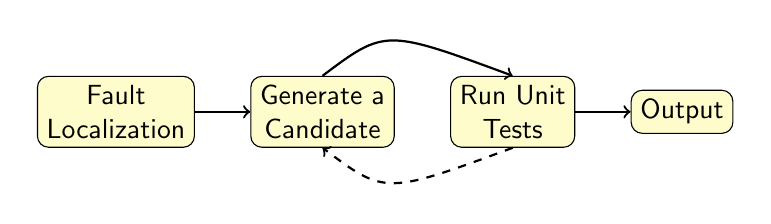
\begin{tikzpicture}[
  font=\sffamily,
  every matrix/.style={ampersand replacement=\&,column sep=2em,row sep=2em},
  box/.style={draw,rounded corners,fill=yellow!20},
  flow/.style={->, thick},
  fail/.style={->, thick, dashed},
  every node/.style={align=center}]
  
% Position the nodes using a matrix layout
\matrix{
      \node[box] (faultLocalization) {Fault \\ Localization};
      \& \node[box] (generateCandidate) {Generate a \\ Candidate};
      \& \node[box] (test) {Run Unit \\ Tests};
      \& \node[box] (output) {Output};
      \\
  };

% Draw the arrows between the nodes and label them.
\draw [flow] (faultLocalization) -- (generateCandidate);
\draw [flow] (generateCandidate.north) .. controls (up:3em) .. (test.north);
\draw [flow] (test) -- (output);
\draw [fail] (test.south) .. controls (down:3em) .. (generateCandidate.south);


% \draw [fail] (oracleInquisition.south) .. controls (down:.5em) and (left:8em) .. (oracleInquisition.west);
% \draw [fail] (collectionOfTestExecutionData) .. controls (down:2em) and (left:9em) .. (oracleInquisition.west);
% \draw [fail] (smtSolving.north) .. controls (down:2em) and (left:10em) .. (oracleInquisition.west);
\end{tikzpicture}

  \end{center}
}